\documentclass[../../manuale-manutentore.tex]{subfiles}

\begin{document}

\subsection{Server}%
\label{sub:installazione/server}

\subsubsection{Installazione Docker}%
\label{subs:installazione_docker}

La prima cosa che l'utente deve fare è verificare l'edizione dell'attuale versione di Windows 10. Aprire la barra di ricerca ed eseguire il comando \bash{winver}.

\begin{figure}[H]
  \centering
  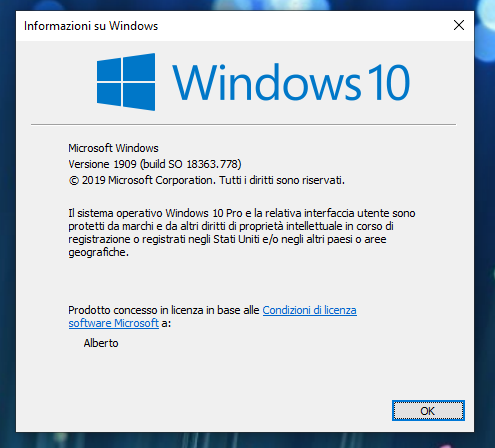
\includegraphics[width=90mm]{winver.png}
  \caption{Risultato winver}%
  \label{fig:risultato_winver}
\end{figure}

Una volta individuata l'edizione, installare:
\begin{description}
  \item[Docker Desktop] se l'edizione di Windows 10 è Professional oppure Enterprise.
  \item[Docker Toolbox] altrimenti.
\end{description}

Nel caso di \textbf{Docker Desktop}, eseguire queste operazioni:
\begin{itemize}
  \item installare l'applicazione Docker Desktop, all'indirizzo \href{https://hub.docker.com/editions/community/docker-ce-desktop-windows}{https://hub.docker.com/editions/community/docker-ce-desktop-windows}.
  \item aprire la barra di ricerca, digitare \textit{Docker Desktop} ed eseguire l'applicazione.
  \item attendere qualche secondo per l'esecuzione di Docker Desktop, poi andare sulla barra delle applicazioni in \textit{Mostra icone risposte} e accertarsi che l'icona dell'applicazione (una balena bianca) sia presente e che, facendo un hover sopra l'icona appaia il messaggio \textit{Docker is running}.
  \item cliccare con il tasto destro sull'icona per aprire il menu, e cliccare sulla voce \textit{Switch to Linux containers} per attivare il daemon Linux con cui la Docker \glossarioLocale{CLI} interagisce e quindi utilizzare i contenitori Linux.
\end{itemize}

Nel caso di \textbf{Docker Toolbox}, seguire i passi per l'installazione dell'applicazione che si trovano all'indirizzo \href{https://docs.docker.com/toolbox/toolbox_install_windows/}{https://docs.docker.com/toolbox/toolbox\_install\_windows/}.
Va precisato che Docker Toolbox esegue Docker in una \glossarioLocale{VM}; di conseguenza i container non sono visibili dall'indirizzo \texttt{localhost}, bensì dall'\glossarioLocale{IP} della VM\@.
Per risolvere questo problema, eseguire queste operazioni per la configurazione del \glossarioLocale{port forwarding}:
\begin{itemize}
  \item selezionare la VM su cui parte Docker (segnato in rosso).
  \item selezionare la voce \textit{Settings} della VM (segnato in arancione scuro).
  \item selezionare la tab \textit{Network} (segnato in arancione chiaro).
  \item cliccare sul pulsante \textit{Port Forwarding} (segnato in arancione scuro).

  \begin{figure}[H]
    \centering
    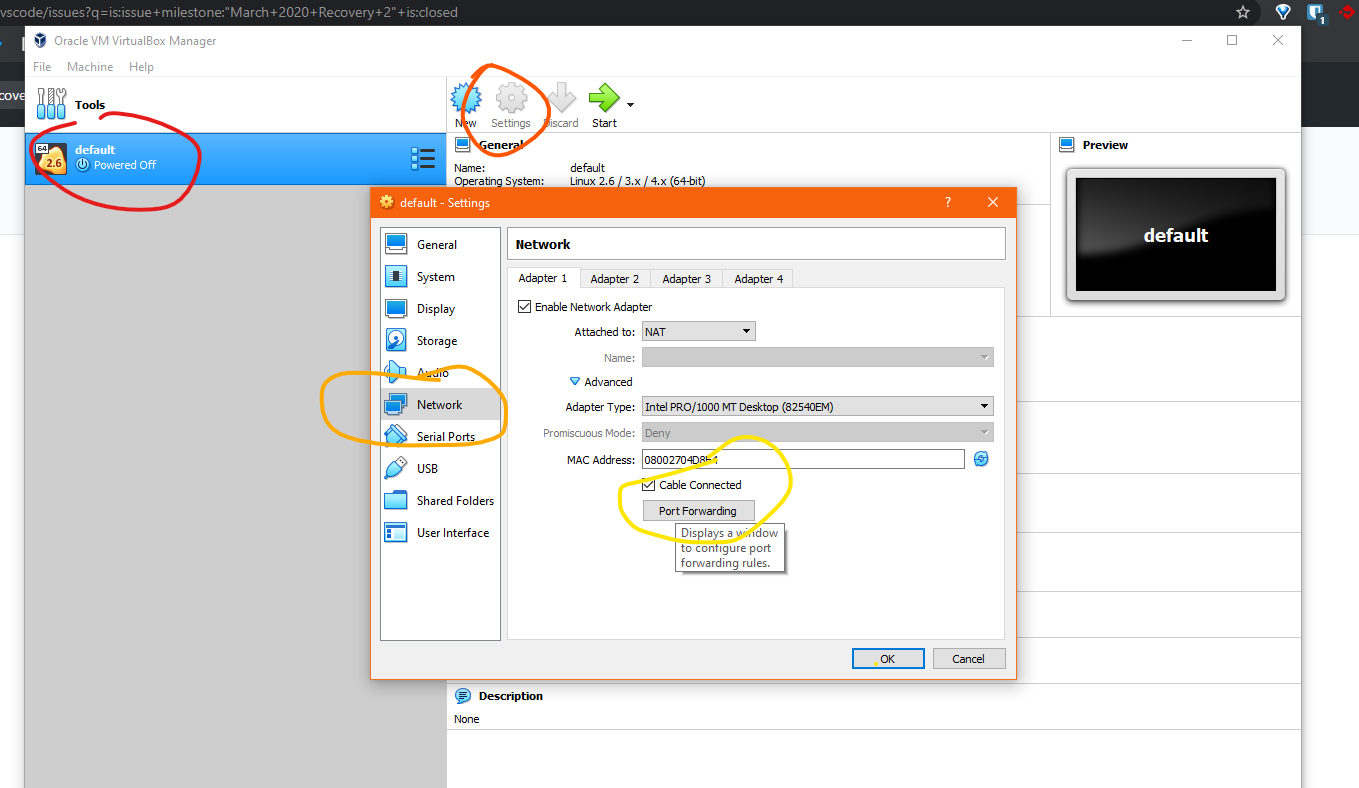
\includegraphics[width=110mm]{virtualbox-port-forwarding-1.png}
    \caption{Port forwarding-Parte 1}%
    \label{fig:port_forwarding_parte_1}
  \end{figure}

  \item aggiungere, se necessario, il nome del servizio con la quale Docker deve comunicare, con annesso tipo di protocollo e le porte, rispettivamente quella pubblicata da VirtualBox (segnata in rosso), e quella pubblicata dal container alla VM (segnata in giallo). Non è necessario che le due porte siano uguali: per dettagli, visitare l'indirizzo \href{https://docs.docker.com/config/containers/container-networking/#published-ports}{https://docs.docker.com/config/containers/container-networking/\#published-ports}.

  \begin{figure}[H]
    \centering
    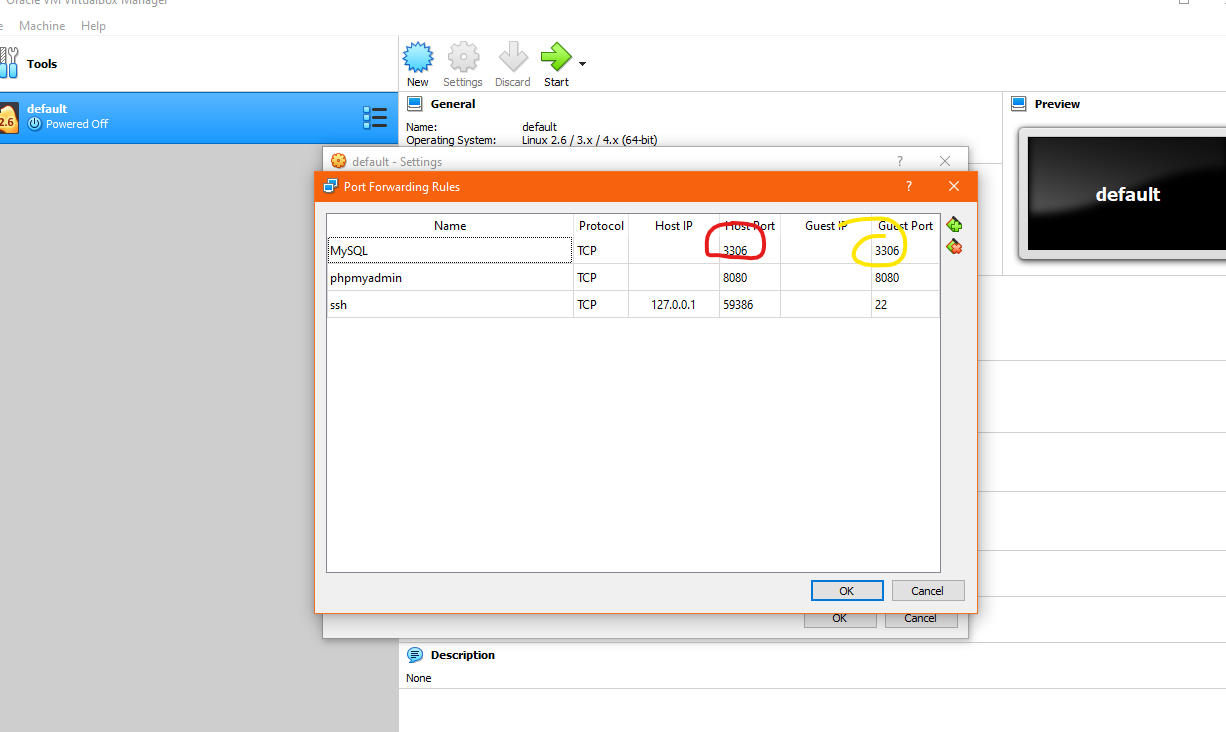
\includegraphics[width=110mm]{virtualbox-port-forwarding-2.png}
    \caption{Port forwarding-Parte 2}%
    \label{fig:port_forwarding_parte_2}
  \end{figure}
\end{itemize}

\subsubsection{Avvio dei servizi}%
\label{subs:avvio_dei_servizi}

Per la gestione delle dipendenze utilizziamo Gradle.
All'interno della repository \href{Gruppone/stalker-server}{Gruppone/stalker-server}, è presente una coppia di script (\texttt{gradlew} per linux e \texttt{gradlew.bat} per Windows) che permette di eseguire i task necessari senza bisogno di installare \glossarioLocale{Gradle}.
Il comando da utilizzare per eseguire il server e renderlo raggiungibile all'indirizzo \texttt{localhost:11111} è:

\begin{minted}{bash}
  ./gradlew bootRun
\end{minted}

Spring utilizza una funzionalità chiamata \glossarioLocale{LiveReload}, che consente la ricompilazione automatica ad ogni modifica del codice sorgente; in questo modo da non è necessario riavviare manualmente il server Spring.\par
Lo strato di persistenza, rappresentato dai database MySQL e InfluxDB, non si attiva automaticamente.
Il comando per avviarlo deve essere eseguito a partire dalla root del server, e un esempio può essere:

\begin{minted}{bash}
  docker-compose up -d rdb
\end{minted}

dove \bash{rdb} (\glossarioLocale{Relational Database}) è il nome del servizio definito all'interno di quei file che rappresenta l'istanza di MySQL\@.
Per conoscere tutti i dettagli dei container che possono essere istanziati, consultare i file \texttt{docker-compose.yml} e \texttt{docker-compose.override.yml}.
È anche possibile far partire più di un servizio alla volta, aggiungendo i nomi dei relativi container nel seguente modo:

\begin{minted}{bash}
  docker-compose up -d rdb rdb-gui
\end{minted}

Questo comando fa partire un'istanza di MySQL e allo stesso tempo un'istanza di \glossarioLocale{PhpMyAdmin}, che è legata al servizio denominato \bash{rdb-gui}.
Esiste un comando generale che fa partire tutti i servizi disponibili:

\begin{minted}{bash}
  docker-compose up -d
\end{minted}

\bash{-d} sta per \bash{--detached} e serve a ritornare il prompt dopo che Docker ha avviato il \glossarioLocale{container}.
Questo comando fa partire allo stesso tempo un'istanza di MySQL, un'istanza di InfluxDB, un'istanza di PhpMyAdmin e un'istanza di \glossarioLocale{Chronograf}, grazie al quale è possibile interagire con i due database attraverso un'interfaccia grafica web, rispettivamente all'indirizzo \texttt{localhost:8080} per PhpMyAdmin, e all'indirizzo \texttt{localhost:8888} per Chronograf. In entrambi i casi, per accedere correttamente vanno utilizzare le credenziali di admin.

Per eseguire il server LDAP, è necessario eseguire il comando:

\begin{minted}{bash}
  cd db/ldap; docker-compose up -d
\end{minted}

La prima parte del comando è necessario per poter avviare correttamente i servizi LDAP, in quanto il caricamento di questi servizi sono separati dal caricamento dello strato di persistenza.
Una volta che l'utente si è posizionato correttamente nella directory, l'utente può avviare tutti i servizi mediante la seconda parte del comando.
In questo caso, il comando fa partire allo stesso tempo un'istanza del server LDAP e un'istanza di \glossarioLocale{PhpLdapAdmin}, grazie al quale è possibile interagire con il server LDAP attraverso un'interfaccia grafica web che visualizza tutti i dati del file \bash{.ldif}, che contiene tutte le utenze autorizzate ad accedere ad esso.
L'indirizzo per connettersi a PhpMyAdmin è \texttt{localhost:8090}, inserendo le credenziali di admin.
Il teardown completo dei servizi che compongono lo strato di persistenza (ovvero lo spegnimento di tutti i container, e quindi di tutti i servizi) si esegue con il comando:

\begin{minted}{bash}
  docker-compose down --rmi all --remove-orphans --volumes
\end{minted}

\end{document}
